%%%%%%%%%%%%%%%%%%%%%%%%%%%%%%%%%%%%%%%%%
% The Legrand Orange Book
% LaTeX Template
% Version 3.1 (February 18, 2022)
%
% This template originates from:
% https://www.LaTeXTemplates.com
%
% Authors:
% Vel (vel@latextemplates.com)
% Mathias Legrand (legrand.mathias@gmail.com)
%
% License:
% CC BY-NC-SA 4.0 (https://creativecommons.org/licenses/by-nc-sa/4.0/)
%
% Compiling this template:
% This template uses biber for its bibliography and makeindex for its index.
% When you first open the template, compile it from the command line with the 
% commands below to make sure your LaTeX distribution is configured correctly:
%
% 1) pdflatex main
% 2) makeindex main.idx -s indexstyle.ist
% 3) biber main
% 4) pdflatex main x 2
%
% After this, when you wish to update the bibliography/index use the appropriate
% command above and make sure to compile with pdflatex several times 
% afterwards to propagate your changes to the document.
%
%%%%%%%%%%%%%%%%%%%%%%%%%%%%%%%%%%%%%%%%%

%----------------------------------------------------------------------------------------
%	PACKAGES AND OTHER DOCUMENT CONFIGURATIONS
%----------------------------------------------------------------------------------------

\documentclass[
	11pt, % Default font size, select one of 10pt, 11pt or 12pt
	fleqn, % Left align equations
	a4paper, % Paper size, use either 'a4paper' for A4 size or 'letterpaper' for US letter size
	%oneside, % Uncomment for oneside mode, this doesn't start new chapters and parts on odd pages (adding an empty page if required), this mode is more suitable if the book is to be read on a screen instead of printed
]{bookSI}

% Book information for PDF metadata, remove/comment this block if not required 
\hypersetup{
	pdftitle={Projekt prenove urnika FOV z APEX}, % Title field
	pdfauthor={Skupina BeeAPEX}, % Author field
	pdfsubject={Razvoj apllikacij}, % Subject field
	pdfkeywords={Malokodno programiranje, APEX, BeeAPEX}, % Keywords
	pdfcreator={LaTeX}, % Content creator field
}

\addbibresource{literature.bib} % Bibliography file

% \definecolor{ocre}{RGB}{243, 102, 25} % Define the color used for highlighting throughout the book
% \definecolor{ocre}{RGB}{54, 88, 162} % blue logo
\definecolor{ocre}{RGB}{248,185,74} % yellow logo


\chapterimage{orange1mod.jpg} % Chapter heading image
\chapterspaceabove{6.5cm} % Default whitespace from the top of the page to the chapter title on chapter pages
\chapterspacebelow{6.75cm} % Default amount of vertical whitespace from the top margin to the start of the text on chapter pages

%----------------------------------------------------------------------------------------

\begin{document}

\selectlanguage{slovene}

%----------------------------------------------------------------------------------------
%	TITLE PAGE
%----------------------------------------------------------------------------------------

\titlepage % Output the title page
	{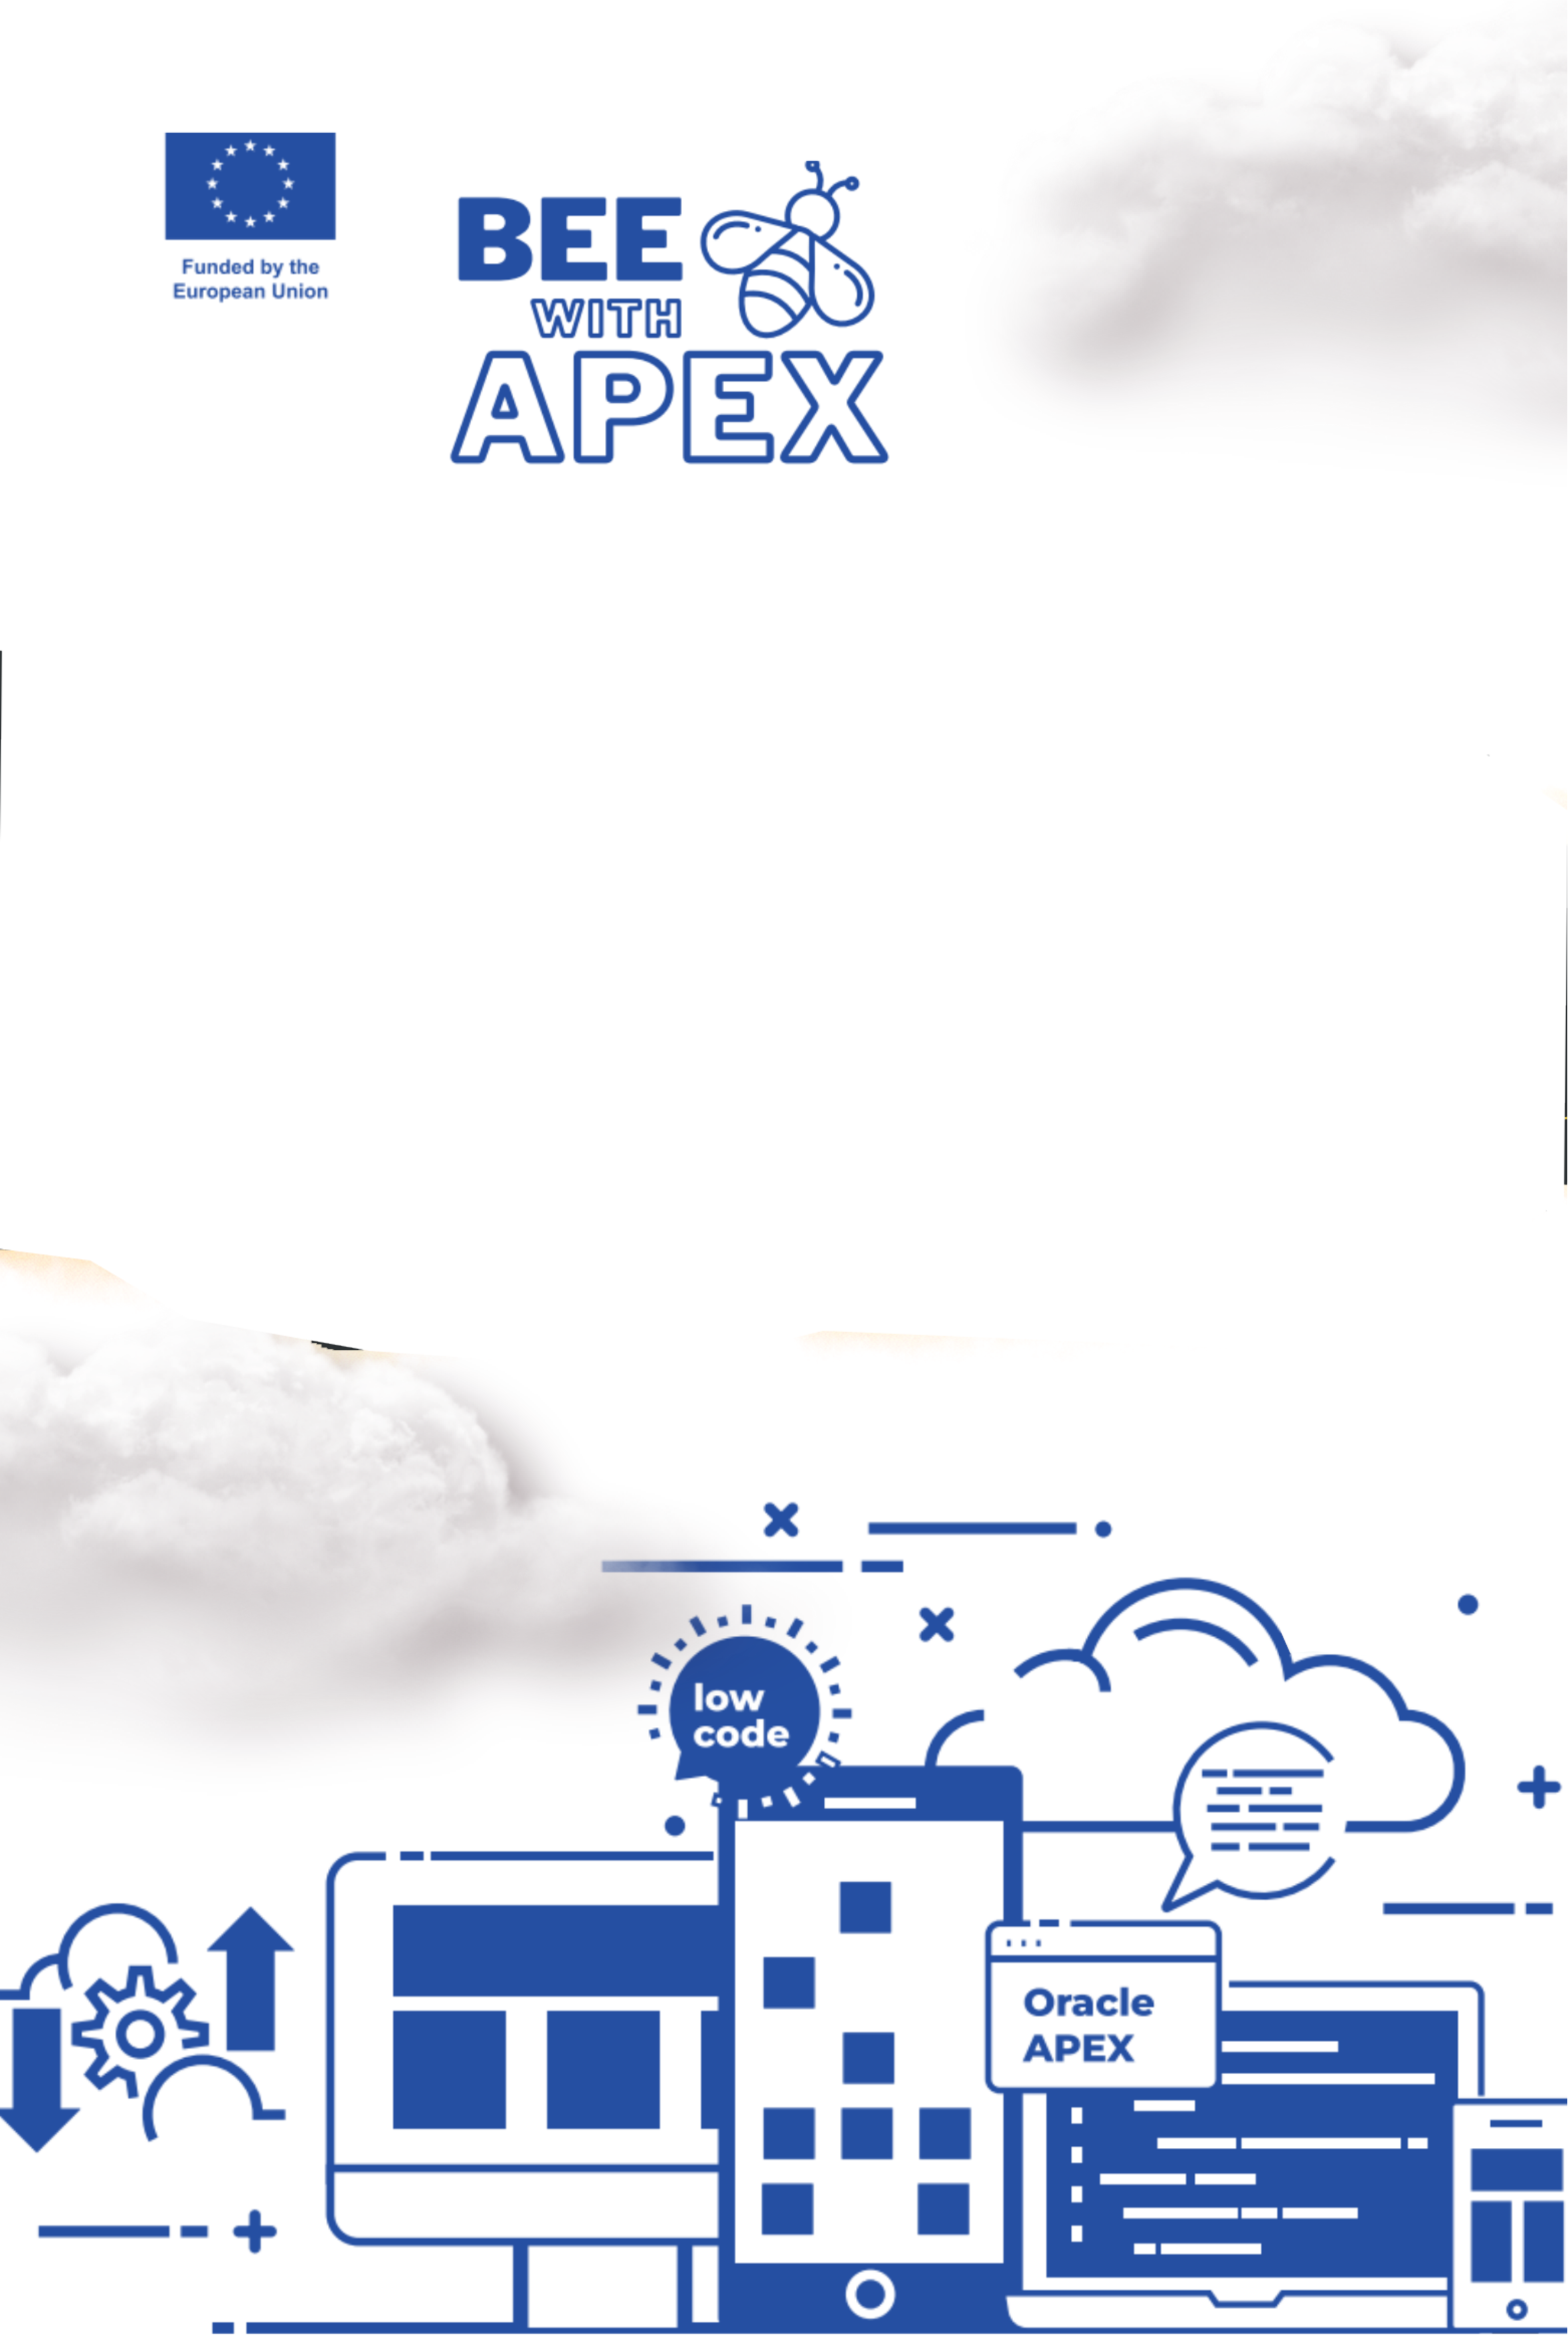
\includegraphics[width=\paperwidth]{background4.pdf}} % Code to output the background image, which should be the same dimensions as the paper to fill the page entirely; leave empty for no background image
	{ % Title(s) and author(s)
		\centering\sffamily % Font styling
		{\Huge\bfseries Poročilo \par Pregled kode v projektu BeeAPEX\par} % Book title
		\vspace{16pt} % Vertical whitespace
		{\LARGE (učbenik, skripti, aplikacije, video vodiči)\par} % Subtitle
		\vspace{24pt} % Vertical whitespace
		{\huge\bfseries Projektna skupina KPO 2023\par} % Author name
	}

%----------------------------------------------------------------------------------------
%	COPYRIGHT PAGE
%----------------------------------------------------------------------------------------

\thispagestyle{empty} % Suppress headers and footers on this page

~\vfill % Push the text down to the bottom of the page

\noindent Avtorske pravice \copyright\ \the\year\, Projektna skupina BeeAPEX\\ % Copyright notice

\noindent \textsc{Izdajatelj: Laboratorij za kakovost in testiranje programske opreme, UM FOV}\\ % Publisher

\noindent \textsc{\href{https://beeapex.eu}{beeapex.eu}}\\ % URL

\noindent To je licencirana vsebina po Creative Commons Attribution-NonCommercial 4.0 License (v nadaljevanju ``Licenca''). Vsebino je dovoljeno uporabljati izključno v skladu z Licenco. Kopija Licence je dostopna na povezavi \url{https://creativecommons.org/licenses/by-nc-sa/4.0}. Razen v primeru, da obstaja zakonska ali pogodbena obveza, je programska oprema po tej Licenci distribuirana po načelu \textsc{``taka, kot je'', brez kakršnihkoli zagotovil ali pogojev}, bodisi, da so ti izraženi implicitno ali ekspilicitno. Preberite Licenco za specifična jezikovna dovoljenja in omejitve.\\

\noindent \textit{1. izdaja, \today } % Printing/edition date

%----------------------------------------------------------------------------------------
%	TABLE OF CONTENTS
%----------------------------------------------------------------------------------------

\pagestyle{empty} % Disable headers and footers for the following pages

\tableofcontents % Output the table of contents

\listoffigures % Output the list of figures, comment or remove this command if not required

\listoftables % Output the list of tables, comment or remove this command if not required

\pagestyle{fancy} % Enable default headers and footers again

\cleardoublepage % Start the following content on a new page
%----------------------------------------------------------------------------------------
%	Acknowledgement and Preface
%----------------------------------------------------------------------------------------
\pagestyle{empty} % Disable headers and footers for the following pages

\chapter*{Zahvala}
\addcontentsline{toc}{chapter}{Zahvala}

Projektni partnerji in projektni tim \href{https://beeapex.eu}{
\includegraphics[scale=0.03]{logo-BeeAPEX-Blue3.png}}:
\begin{itemize}
	\item \href{https://www.um.si/en/home-page}{Univerza Maribor} \href{https://fov.um.si/en}{Fakulteta za organizacijske vede,} 
	\item \href{http://www.unizg.hr/homepage}{Univerza Zagreb} \href{https://www.foi.unizg.hr/en}{Fakulteta za organizacijo in informatiko,}
	\item \href{https://www.uniza.sk/index.php/en/}{Univerza Žilina,} 
	\item \href{https://www.kozminski.edu.pl/en}{Univerza Kozminski,}
	\item \href{https://www.ihu.gr/en/enhome}{Mednarodna grška univerza in }
	\item \href{https://www.jku.at/en}{Univerza Johannes Kepler}	
\end{itemize}	
se zahvaljujemo za finančno podporo 
\includegraphics[scale=0.15]{logo-ce-horizontal-en-quadri-lr.png} z akcijo Erasmus + Better Employability for Everyone with APEX (projekt ID 2021-1-SI01-KA220-HED-000032218), ki ga financira program Erasmus+ programme Evropske unije. 

Podpora Evropske komisije za izdelavo te publikacije ne pomeni odobritve vsebine. Ta odraža samo stališča avtorjev. Komisija ne more biti odgovorna za kakršno koli uporabo informacij, ki jih publikacija vsebuje.
\newline

\vspace{1cm}
\noindent \textit{Posebej se zahvaljujejemo tudi:}
\begin{itemize}
	\item gospodu \textit{Darku Jurekoviću, programskemu vodji} \href{https://academy.oracle.com}{Oracle Academy} za njegovo nenehno pomoč pri širjenju rezultatov projekta in 
	\item gospodu \textit{Aljažu Maliju, direktorju podjetja} \href{https://www.right-thing.solutions/ords/r/app/en/home}{THE RIGHT THING SOLUTIONS} za dragocene nasvete o APEX-u pred in med projektom.	
\end{itemize}

\vspace{1cm}
\noindent \textit{Projektna skupina KPO 2023}

\chapter*{Predgovor}
\addcontentsline{toc}{chapter}{Predgovor}


\vspace{1cm}
\indent Dobrodošli pri raziskovanju Oracle Application Express (APEX) – intuitivne in zmogljive razvojne malokodne platforme za ustvarjanje podatkovno vodenih spletnih aplikacij. Ta učbenik je zasnovan z namenom, da vas obogati s kompetencami za izkoriščanje celotnega potenciala Oracle APEX in izdelavo vrhunskih aplikacij za reševanje resničnih poslovnih izzivov.
\vspace{0.5cm}

\noindent Del I v učbeniku je naslovljen ``Kako delate v APEX-u?''. Obravnava osnovne vidike tega orodja. V dvanajstih poglavjih boste potovali po vsebinah, ki vam bodo omogočile razumevanje jedrnih konceptov, pridobitev študijskega razvojnega okolja ter spoznavanje različnih funkcij pri gradnji robustnih aplikacij. Vsako poglavje obravnava specifično temo, zagotavlja jasna navodila ter vabi k preskusu za boljšo učno izkušnjo.

Poglavje 1: ``Kako začnete z Oracle APEX?'' razloži kaj je, za kaj se uporablja in več načinov za pripravo študijskega okolja za učenje in razvijanje aplikacij.

Poglavje 2: ``Kako pripravite bazo podatkov?'' podaja uvod v modeliranje podatkov, upravljanje baze podatkov, manipuliranje podatkov ter poizvedovanje. Za začetnike so predstavljeni vsi pomembno koncepti modeliranja podatkov, ki je obvezna veščina.

Poglavje 3: ``Kako navigirate v APEX-u?'' popelje bralca po funkcijah APEX-a, ki omogočajo razvoj aplikacij, generiranje in prilagajanje različnih spletnih strani in njihovih komponent. Izvajanje in testiranje aplikacije je samo en zavihek oddaljeno od razvojnega okolja.

Poglavje 4: ``Kako izmenjujete podatke v APEX-u?'' daje vpogled v zmogljivosti izvažanja in uvažanja podatkov. Poglavje prikazuje izmenjav z datotekami, preglednicami in tudi s pomočjo storitve RESTful. 

Poglavje 5: ``Kako izdelate prvi osnutek aplikacije?'' vabi k preskusu razvojnih zmogljivosti platforme APEX. Ugotovili boste, da po odločitvi glede vaših podatkov, lahko nemudoma generirate prikupno in uporabno aplikacijo brez programiranja. Razloži vam kako kontrolirano dodeljujete dostopne pravice različnim vlogam uporabnikov s čarovnikom.

Poglavje 6: ``Kako uredite poročila?'' vodi skozi različne vpoglede v podatke od klasičnih poročil do interaktivnih poročil. APEX ima vgrajene funkcije, ki končnemu uporabniku omogočajo prilagajanje brez programiranje ali posredovanja razvijalca.

Poglavje 7: ``Kako uredite obrazce?'' vas uvede v tri splošne tipe spletnih obrazcev, vključno z zahtevnejšimi, ki imajo glavo in podrobnosti. Prilagajanje in generiranje spletnih obrazcev ne bo zahtevalo nobenega programiranja. 

Poglavje 8: ``Kako poročila spremenite v grafikone?'' vas popelje po funkcijah APEX-a, ki omogočajo prikaz podatkov v obliki različnih grafikonov naravnost iz besedilnih poročil.

Poglavje 9: ``Kako urejate menije?'' predstavlja različne navigacijske elemente v APEX-u.

Poglavje 10: ``Kako sodelujete v timu?'' daje vpogled v zmogljivosti APEX-a za podporo dela skupine, kajti zelo redko se zgodi, da na razvoju aplikacije dela zgolj en razvijalec.

Poglavje 11: ``Kako izkoristite galerijo aplikacij in vtičnikov?'' prikazuje moč APEX-a za ponovno uporabo dobrih vzorov.

Poglavje 12: ``Kako upravljate paketne in večjezične aplikacije?'' vas popelje na pot distribucije vaše aplikacije v drugo APEX-ovo okolje z uporabniki, ki govorijo druge jezike.

Del I pokriva tudi vsebine, ki so ključne za varnost aplikacij, strategije namestitev in pripravo za produkcijsko uporabo.

\vspace{0.5cm}
\noindent Del II tega učbenika vas popelje onkraj osnov in predstavi dvanajst privlačnih poslovnih primerov od besednega opisa, preko vseh tehničnih podrobnosti do rešitve - aplikacije. Vsak primer je skrbno dokumentiran, da zagotovi celovito razumevanje razvoja aplikacij z vidika poslovanja, podatkov in uporabniškega vmesnika. Ta del vključuje primere aplikacij za podjetja:
\begin{itemize}
	\item intranetne novice za zaposlene, 
	\item sistem malih inovacij, 
	\item vodenje poslovnih procesov z delovnimi tokovi, 	
	\item kalkulacija materialne kosovnice, 	
	\item sistem za ocenjevanje knjig, 	
	\item vodenje prehrane in diete,	 
	\item razporejanje uradnih ur, 	
	\item zaračunavanje storitev v telekomunikacijskem podjetju, 	
	\item najemanje vozil
\end{itemize}   
za skupine, društva:
\begin{itemize}
	\item katalog rastlin, 
	\item izmenjava rastlin
\end{itemize} 
ter splošno uporabno avtorizacijo in upravljanje uporabnikov.
\noindent V vsakem poslovnem primeru so vključeni:
\begin{itemize}
	\item Poslovni pogled na primer: pregled poslovne situacije.
	\item Definicija problema: iskanje odgovora na kdo in zakaj ima nekdo glavobol.
	\item Primeri uporabe: predstavljene so tri vrste opisov: besedni, polstrukturirani in grafični za pripravo dokumentacije primerov uporabe v UML.
	\item Logični in relacijski podatkovni model: APEX ima vse funkcije za zagon aplikacije iz novih podatkovnih struktur, uporabo in spreminjanje obstoječih, združevanje z drugimi orodji za modeliranje podatkov in podporo za vnaprejšnjega ali obratnega inženiringa. Prizadevanja razvijalcev, da bi zagotovili ustrezne dele podatkov in povezave med njimi ter upoštevanje poslovnih potreb, so osnova za oblikovanje uporabniških vmesnikov.	
	\item Aplikacijski vmesniki: učbenik ponuja HTML strani, poročila, obrazce, polja, menije, gumbe in hiperpovezave, ki materializirajo poslovno situacijo, rešitev poslovnega problema, primere uporabe in podatke z mislijo na končnega uporabnika.
	\item Dodatno učno gradivo: za izboljšanje, pospešitev in pomoč na razvojni poti boste našli povezave do izvoženih paketnih aplikacij, skriptov, podatkov in video vodičev za vsako poglavje. Ti viri vam bodo zagotovili praktične vpoglede, kar vam bo omogočilo, da okrepite svoje znanje in ga neposredno uporabite v projektih iz resničnega sveta.
\end{itemize}

\noindent Ne glede na to, ali ste izkušen razvijalec, ki želi še povečati svoje kompetence, ali začetnik, ki želi raziskati svet APEX-a, je ta učbenik vaš dober vodnik. Upamo, da ga bodo tudi tisti, ki se ne učijo IT, našli kot neprecenljivega spremljevalca na poti do obvladovanja Oracle APEX in gradnje inovativnih aplikacij, ki imajo pozitiven učinek. 

\vspace{0.5cm}
\noindent Učbenik in dodatno študijsko gradivo so zasnovani za približno 75 ur napora študenta (3 ECTS). Upamo, da bodo omogočili različne načine študija:
\begin{itemize}
	\item tečaj ali predmet, pri katerem učitelj predava in izvaja laboratorijske vaje,
	\item mešano učenje (to je del vodi učitelj, del samostojno preštudira študent) in tudi
	\item popolnoma samostojen študij.
\end{itemize}

\noindent Glede na osnovno znanje študentov in razpoložljiv čas za izvajanje tečaja/predmeta lahko učitelji enostavno sestavijo nabor poglavij, ki ustrezajo učnim situacijam, kot so: izvenštudijski tečaji/predmeti, poletne šole, časovno omejeni dogodki za predstavitve malokodnega pristopa za vse študente (ne samo v IT ali računalničarje) in praktično usposabljanje v različnih panogah industrije.

\vspace{0.5cm}
\noindent Za razvoj učbenika in dopolnilnih študijskih gradiv smo uporabljali verziji APEX-a 22 in 23. Avtorji smo prepričani, da bodo razloženi in uporabljeni koncepti ter jedrne tehnologije zelo koristile študentom tudi v prihodnjih verzijah APEX-a.
\newline
\vspace{1cm}
\noindent Uživajte v uporabi čarovnikov in malokodnega programiranja!
\newline

\vspace{1cm}
\noindent red. prof. dr. Robert Leskovar\\
vodja projekta BeeAPEX, predstojnik Katedre za informatiko Fakultete za organizacijske vede UM



\pagestyle{fancy} % Enable default headers and footers again
%----------------------------------------------------------------------------------------
%	PART 1
%----------------------------------------------------------------------------------------

%\part{Kako delate v APEX-u?}

%----------------------------------------------------------------------------------------
%	SECTIONING EXAMPLES CHAPTER
%----------------------------------------------------------------------------------------

\chapterimage{orange2mod.jpg} % Chapter heading image
\chapterspaceabove{6.75cm} % Whitespace from the top of the page to the chapter title on chapter pages
\chapterspacebelow{7.25cm} % Amount of vertical whitespace from the top margin to the start of the text on chapter pages

%------------------------------------------------
%\include{./Include/Tex/ch01SI}
%\include{./Include/Tex/ch02SI} 
%\include{./Include/Tex/ch03SI}
%\include{./Include/Tex/ch04SI}
%\include{./Include/Tex/ch05SI}
%\include{./Include/Tex/ch06SI}
%\include{./Include/Tex/ch07SI}
%\include{./Include/Tex/ch08SI}
%\include{./Include/Tex/ch09SI}
%\include{./Include/Tex/ch10SI}
%\include{./Include/Tex/ch11SI}
%\include{./Include/Tex/ch12SI}

%----------------------------------------------------------------------------------------
%	PART 2
%----------------------------------------------------------------------------------------

\part{Poglavja}

%----------------------------------------------------------------------------------------
%	From zero to application
%----------------------------------------------------------------------------------------
\chapter{Intranetne novice za zaposlene}\label{chap13SI}
\chapterauthor{R. Leskovar, U. Rajkovič, A.Baggia; prevod R. Leskovar}
%% each chapter must have the following sections
%% - Business view of the case
%% - Problem definition (and requirement specification)
%% - Use cases
%% - Data model
%% - Application interfaces
%% If you need deeper structure use \subsection{title} and \subsubsection{title}
%% Latex commands for creating various lists and tables are:
%% - \begin{itemize} \item ... \end{itemize} or \begin{enumerate} 	\item .. \end{enumerate}
%% - \begin{table} 	\caption{ } \label{key} \begin{tabular}{cols} \end{tabular}content... \end{table}
%% e.g.
%% \begin{table}
	%% 	\caption{Mean growth rate and intakes
		%% 		of supplement, milk, and water for 4 diets.}
	%% 	\label{dietgrowth}\centering
	%% 	\begin{tabular}{|l|r|r|r|r|}\hline
		%% 		&Growth&Supplement&Milk&Water\\
		%% 		Supplement&rate&intake&intake&intake\\
		%% 		&(g/day)&(g/day)&(ml/kg$^{0.75}$)&
		%% 		(ml/kg$^{0.75}$)\\\hline
		%% 		Lucerne &145&450&10.5&144\\\hline
		%% 		Sesbania&132&476& 9.2&128\\\hline
		%% 		Leucaena&128&364& 8.9&121\\\hline
		%% 		None & 89& 0& 9.8&108\\\hline
		%% 	\end{tabular}
	%% \end{table}

\section{Učbenik}
\subsection{Zaznamki Robert Leskovar}
V učbeniku (poglavje \ref{chap13SI}) so naslednje pomanjkljivosti - to je samo demosntracija:
\begin{itemize}
	\item stran 225: napaka pri besedi XZ; pravilno je XY
	\item stran 225: namesto besedila \textit{Sprememba postopka objavljanja in nova platforma } mora biti \textbf{Sprememba postopka in platforma }...
	\item n	
\end{itemize}

\section{Skripti}
\subsection{Zaznamki osebe xy1}
Primer naštevanja:
\begin{itemize}
	\item ena
	\item ...
	\item n	
\end{itemize}

\section{Aplikacija}
\subsection{Zaznamki osebe xy1}
Primer naštevanja:
\begin{itemize}
	\item ena
	\item ...
	\item n	
\end{itemize}

\section{Video vodič}
\subsection{Zaznamki osebe xy1}
Primer naštevanja:
\begin{itemize}
	\item ena
	\item ...
	\item n	
\end{itemize}
\chapter{GreenDi - katalog rastlin}\label{chapSI14}
\chapterauthor{Vjeran Strahonja, Dijana Oreški, Darko Andročec, Ana Kutnjak; prevod R. Leskovar }

\section{Učbenik}
\subsection{Zaznamki osebe xy1}
Primer naštevanja:
\begin{itemize}
	\item ena
	\item ...
	\item n	
\end{itemize}

\section{Skripti}
\subsection{Zaznamki osebe xy1}
Primer naštevanja:
\begin{itemize}
	\item ena
	\item ...
	\item n	
\end{itemize}

\section{Aplikacija}
\subsection{Zaznamki osebe xy1}
Primer naštevanja:
\begin{itemize}
	\item ena
	\item ...
	\item n	
\end{itemize}

\section{Video vodič}
\subsection{Zaznamki osebe xy1}
Primer naštevanja:
\begin{itemize}
	\item ena
	\item ...
	\item n	
\end{itemize} 
\chapter{GreenDi - avtorizacija in upravljanje uporabnikov}\label{chap15SI}
\chapterauthor{Vjeran Strahonja; prevod R. Leskovar}

\section{Učbenik}
\subsection{Zaznamki osebe xy1}
Primer naštevanja:
\begin{itemize}
	\item ena
	\item ...
	\item n	
\end{itemize}

\section{Skripti}
\subsection{Zaznamki osebe xy1}
Primer naštevanja:
\begin{itemize}
	\item ena
	\item ...
	\item n	
\end{itemize}

\section{Aplikacija}
\subsection{Zaznamki osebe xy1}
Primer naštevanja:
\begin{itemize}
	\item ena
	\item ...
	\item n	
\end{itemize}

\section{Video vodič}
\subsection{Zaznamki osebe xy1}
Primer naštevanja:
\begin{itemize}
	\item ena
	\item ...
	\item n	
\end{itemize}
\chapter{Sistem malih inovacij}\label{chap16SI}
\chapterauthor{R. Leskovar, U. Rajkovič, A.Baggia; prevod R. Leskovar}
%% each chapter must have the following sections
%% - Business view of the case
%% - Problem definition (and requirement specification)
%% - Use cases
%% - Data model
%% - Application interfaces
%% If you need deeper structure use \subsection{title} and \subsubsection{title}
%% Latex commands for creating various lists and tables are:
%% - \begin{itemize} \item ... \end{itemize} or \begin{enumerate} 	\item .. \end{enumerate}
%% - \begin{table} 	\caption{ } \label{key} \begin{tabular}{cols} \end{tabular}content... \end{table}
%% e.g.
%% \begin{table}
%% 	\caption{Mean growth rate and intakes
%% 		of supplement, milk, and water for 4 diets.}
%% 	\label{dietgrowth}\centering
%% 	\begin{tabular}{|l|r|r|r|r|}\hline
%% 		&Growth&Supplement&Milk&Water\\
%% 		Supplement&rate&intake&intake&intake\\
%% 		&(g/day)&(g/day)&(ml/kg$^{0.75}$)&
%% 		(ml/kg$^{0.75}$)\\\hline
%% 		Lucerne &145&450&10.5&144\\\hline
%% 		Sesbania&132&476& 9.2&128\\\hline
%% 		Leucaena&128&364& 8.9&121\\\hline
%% 		None & 89& 0& 9.8&108\\\hline
%% 	\end{tabular}
%% \end{table}

\section{Učbenik}
\subsection{Zaznamki osebe xy1}
Primer naštevanja:
\begin{itemize}
	\item ena
	\item ...
	\item n	
\end{itemize}

\section{Skripti}
\subsection{Zaznamki osebe xy1}
Primer naštevanja:
\begin{itemize}
	\item ena
	\item ...
	\item n	
\end{itemize}

\section{Aplikacija}
\subsection{Zaznamki osebe xy1}
Primer naštevanja:
\begin{itemize}
	\item ena
	\item ...
	\item n	
\end{itemize}

\section{Video vodič}
\subsection{Zaznamki osebe xy1}
Primer naštevanja:
\begin{itemize}
	\item ena
	\item ...
	\item n	
\end{itemize}
\chapter{Vodenje poslovnih procesov} \index{vodenje poslovnih procesov}\label{chap17SI}
\chapterauthor{R. Leskovar, U. Rajkovič, A.Baggia; prevod R. Leskovar}

\section{Učbenik}
\subsection{Zaznamki osebe xy1}
Primer naštevanja:
\begin{itemize}
	\item ena
	\item ...
	\item n	
\end{itemize}

\section{Skripti}
\subsection{Zaznamki osebe xy1}
Primer naštevanja:
\begin{itemize}
	\item ena
	\item ...
	\item n	
\end{itemize}

\section{Aplikacija}
\subsection{Zaznamki osebe xy1}
Primer naštevanja:
\begin{itemize}
	\item ena
	\item ...
	\item n	
\end{itemize}

\section{Video vodič}
\subsection{Zaznamki osebe xy1}
Primer naštevanja:
\begin{itemize}
	\item ena
	\item ...
	\item n	
\end{itemize}
\chapter{GreenDi – menjava rastlin in semen}\label{chapSI18}
\chapterauthor{Vjeran Strahonja, Dijana Oreški, Darko Andročec, Ana Kutnjak; prevod R. Leskovar}

\section{Učbenik}
\subsection{Zaznamki osebe xy1}
Primer naštevanja:
\begin{itemize}
	\item ena
	\item ...
	\item n	
\end{itemize}

\section{Skripti}
\subsection{Zaznamki osebe xy1}
Primer naštevanja:
\begin{itemize}
	\item ena
	\item ...
	\item n	
\end{itemize}

\section{Aplikacija}
\subsection{Zaznamki osebe xy1}
Primer naštevanja:
\begin{itemize}
	\item ena
	\item ...
	\item n	
\end{itemize}

\section{Video vodič}
\subsection{Zaznamki osebe xy1}
Primer naštevanja:
\begin{itemize}
	\item ena
	\item ...
	\item n	
\end{itemize}
\chapter{Sistem za ocenjevanje knjig}\label{chap19SI}
\chapterauthor{A. Kutnjak, L. Hrustek, A. Baggia and R.Leskovar; prevod R. Leskovar}

\section{Učbenik}
\subsection{Zaznamki osebe xy1}
Primer naštevanja:
\begin{itemize}
	\item ena
	\item ...
	\item n	
\end{itemize}

\section{Skripti}
\subsection{Zaznamki osebe xy1}
Primer naštevanja:
\begin{itemize}
	\item ena
	\item ...
	\item n	
\end{itemize}

\section{Aplikacija}
\subsection{Zaznamki osebe xy1}
Primer naštevanja:
\begin{itemize}
	\item ena
	\item ...
	\item n	
\end{itemize}

\section{Video vodič}
\subsection{Zaznamki osebe xy1}
Primer naštevanja:
\begin{itemize}
	\item ena
	\item ...
	\item n	
\end{itemize}
\chapter{Materialna kosovnica in kalkulacija stroškov}\index{materialna kosovnica}\label{chap20SI}
\chapterauthor{R. Leskovar, U. Rajkovič, A.Baggia; prevod R. Leskovar}

\section{Učbenik}
\subsection{Zaznamki osebe xy1}
Primer naštevanja:
\begin{itemize}
	\item ena
	\item ...
	\item n	
\end{itemize}

\section{Skripti}
\subsection{Zaznamki osebe xy1}
Primer naštevanja:
\begin{itemize}
	\item ena
	\item ...
	\item n	
\end{itemize}

\section{Aplikacija}
\subsection{Zaznamki osebe xy1}
Primer naštevanja:
\begin{itemize}
	\item ena
	\item ...
	\item n	
\end{itemize}

\section{Video vodič}
\subsection{Zaznamki osebe xy1}
Primer naštevanja:
\begin{itemize}
	\item ena
	\item ...
	\item n	
\end{itemize}
\chapter{Vodenje prehrane in diete}\label{chapSI21}
\chapterauthor{A. Angeioplastis, G. Myllis, A. Tsimpiris, D. Varsamis; prevod R. Leskovar}

\section{Učbenik}
\subsection{Zaznamki osebe xy1}
Primer naštevanja:
\begin{itemize}
	\item ena
	\item ...
	\item n	
\end{itemize}

\section{Skripti}
\subsection{Zaznamki osebe xy1}
Primer naštevanja:
\begin{itemize}
	\item ena
	\item ...
	\item n	
\end{itemize}

\section{Aplikacija}
\subsection{Zaznamki osebe xy1}
Primer naštevanja:
\begin{itemize}
	\item ena
	\item ...
	\item n	
\end{itemize}

\section{Video vodič}
\subsection{Zaznamki osebe xy1}
Primer naštevanja:
\begin{itemize}
	\item ena
	\item ...
	\item n	
\end{itemize}
\chapter{Razporejanje uradnih ur} \index{Razporejanje uradnih ur}\label{chapEN22}
\chapterauthor{J. Mańko, M. Sońta, R. Leskovar; prevod R. Leskovar}

\section{Učbenik}
\subsection{Zaznamki osebe xy1}
Primer naštevanja:
\begin{itemize}
	\item ena
	\item ...
	\item n	
\end{itemize}

\section{Skripti}
\subsection{Zaznamki osebe xy1}
Primer naštevanja:
\begin{itemize}
	\item ena
	\item ...
	\item n	
\end{itemize}

\section{Aplikacija}
\subsection{Zaznamki osebe xy1}
Primer naštevanja:
\begin{itemize}
	\item ena
	\item ...
	\item n	
\end{itemize}

\section{Video vodič}
\subsection{Zaznamki osebe xy1}
Primer naštevanja:
\begin{itemize}
	\item ena
	\item ...
	\item n	
\end{itemize}
\chapter{Primer telekomunikacijskih storitev}\index{telekomunikacijske storitve}\label{chap23SI}
\chapterauthor{Veronika Šalgová, Jozef Kostolný, Michal Mrena, Michal Kvet, Miroslav Potočár; prevod R. Leskovar}

\section{Učbenik}
\subsection{Zaznamki osebe xy1}
Primer naštevanja:
\begin{itemize}
	\item ena
	\item ...
	\item n	
\end{itemize}

\section{Skripti}
\subsection{Zaznamki osebe xy1}
Primer naštevanja:
\begin{itemize}
	\item ena
	\item ...
	\item n	
\end{itemize}

\section{Aplikacija}
\subsection{Zaznamki osebe xy1}
Primer naštevanja:
\begin{itemize}
	\item ena
	\item ...
	\item n	
\end{itemize}

\section{Video vodič}
\subsection{Zaznamki osebe xy1}
Primer naštevanja:
\begin{itemize}
	\item ena
	\item ...
	\item n	
\end{itemize}
\chapter{Najem vozila} \index{najem vozila, rent-a-car} \label{chapEN24}
\chapterauthor{A. Angeioplastis, G. Myllis, A. Tsimpiris, D. Varsamis; prevod R. Leskovar}

\section{Učbenik}
\subsection{Zaznamki osebe xy1}
Primer naštevanja:
\begin{itemize}
	\item ena
	\item ...
	\item n	
\end{itemize}

\section{Skripti}
\subsection{Zaznamki osebe xy1}
Primer naštevanja:
\begin{itemize}
	\item ena
	\item ...
	\item n	
\end{itemize}

\section{Aplikacija}
\subsection{Zaznamki osebe xy1}
Primer naštevanja:
\begin{itemize}
	\item ena
	\item ...
	\item n	
\end{itemize}

\section{Video vodič}
\subsection{Zaznamki osebe xy1}
Primer naštevanja:
\begin{itemize}
	\item ena
	\item ...
	\item n	
\end{itemize}


%----------------------------------------------------------------------------------------

\stopcontents[part] % Manually stop the 'part' table of contents here so the previous Part page table of contents doesn't list the following chapters

%----------------------------------------------------------------------------------------
%	BIBLIOGRAPHY
%----------------------------------------------------------------------------------------

\chapterimage{} % Chapter heading image
\chapterspaceabove{2.5cm} % Whitespace from the top of the page to the chapter title on chapter pages
\chapterspacebelow{2cm} % Amount of vertical whitespace from the top margin to the start of the text on chapter pages

%------------------------------------------------

\chapter*{Literatura}
\markboth{\sffamily\normalsize\bfseries Literatura}{\sffamily\normalsize\bfseries Literatura} % Set the page headers to display a Bibliography chapter name
\addcontentsline{toc}{chapter}{\textcolor{ocre}{Literatura}} % Add a Bibliography heading to the table of contents

\section*{Članki}
\addcontentsline{toc}{section}{Članki} % Add the Articles subheading to the table of contents

% set language for specific edition. There is no slovene quote style, use french instead
\setquotestyle{croatian}
\printbibliography[heading=bibempty, type=article] % Output article bibliography entries

\section*{Knjige}
\addcontentsline{toc}{section}{Knjige} % Add the Books subheading to the table of contents

\printbibliography[heading=bibempty, type=book] % Output book bibliography entries

%----------------------------------------------------------------------------------------
%	INDEX
%----------------------------------------------------------------------------------------

\cleardoublepage % Make sure the index starts on an odd (right side) page
\phantomsection
\addcontentsline{toc}{chapter}{\textcolor{ocre}{Stvarno kazalo}} % Add an Index heading to the table of contents
\printindex % Output the index

%----------------------------------------------------------------------------------------
%	APPENDICES
%----------------------------------------------------------------------------------------

\chapterimage{orange2mod.jpg} % Chapter heading image
\chapterspaceabove{6.75cm} % Whitespace from the top of the page to the chapter title on chapter pages
\chapterspacebelow{7.25cm} % Amount of vertical whitespace from the top margin to the start of the text on chapter pages

%\begin{appendices}

%\renewcommand{\chaptername}{Dodatek} % Change the chapter name to Appendix, i.e. "Appendix A: Title", instead of "Chapter A: Title" in the headers


%------------------------------------------------
%\include{./Include/Tex/appenddix01SI}
%\include{./Include/Tex/appenddix02EN}
%\include{./Include/Tex/appenddix03EN}
%------------------------------------------------
%\end{appendices}

%----------------------------------------------------------------------------------------

\end{document}
